\input{/Users/daniel/github/config/preamble.sty}

\begin{document}

\begin{minipage}{\textwidth}
	\begin{minipage}{1\textwidth}
		Geometry of Algebraic Varieties \hfill Daniel González Casanova Azuela
		
		{\small\hfill\href{https://github.com/danimalabares/ag}{github.com/danimalabares/ag}}
	\end{minipage}
\end{minipage}\vspace{.2cm}\hrule

\vspace{10pt}

{\Huge Exercises in algebraic geometry}

If not explicity stated, exercises are from Hartshorne.

\tableofcontents

\section{Chapter I}

\subsection{No\c c\~oes b\'asicas}

\begin{itemize}
	\item Ussando que $\mathbb{R}=k[x_1,\ldots,x_n]$ \'e Noetheriano (=todo ideal \'e finitamente generado), vimos que todo aberto de Zariski \'e uma uni\~ao finita de conjuntos da forma.

	\item Se $X\subseteq \mathbb{A}^{n} $ \'e uma variedade afim (=existe $\mathfrak{a}\subset R$ tal que $X=\mathbb{V}(\mathfrak{a})$), os conjuntos fechados de $X$ s\~ao $\mathbb{V}(\mathfrak{b})\cap \mathbb{V}(\mathfrak{a})=\mathbb{V}(\mathfrak{a}+\mathfrak{b})$
	
	\item Nullstellenstz fraco:
		\[\operatorname{Spm }(R):=\{\text{ideais maximais de $R$} \} =\{\left<x_1-a_1,\ldots,x_n-a_n\right> :a_i\in k\}\]

	\item Nullstellensatz:
		\[\mathbb{I}(\mathbb{V}(\mathfrak{a}))=\sqrt{\mathbb{a}} \qquad \mathbb{V}(\mathbb{I}(S))=\overline{S}\]

	\item Corol\'ario:

		\[\begin{tikzcd}
			\{\text{affine varieties of $\mathbb{A}^{n} $} \} \arrow[r,"1-1"]&\{\text{radical ideals of $R$} \} \\
			\{\text{irreducible varieties of $\mathbb{A}^{n} $} \}\arrow[r]&\arrow[l]\operatorname{Spec}(R)=\{\text{ideais primos} \} \\
			\{\text{pontos de $\mathbb{A}^{n} $} \} \arrow[r]&\arrow[l]\operatorname{Spm}(R)
		\end{tikzcd}\]
	
	\item Para duas variedades $X\subseteq \mathbb{A}^n$, $Y\subseteq \mathbb{A}^m$,
		\[\operatorname{Hom}(X,Y)=\{\varphi:X\to Y|\exists \tilde{\varphi}=(f_1,\ldots,f_m), f_i\in R \}\]
		e as $f_i$ extendem a $\varphi$.

		 \item Tem uma equival\^encia de categorias
			 \[(\text{affine alg. varieties})^{\operatorname{op}}\to \text{reduced f.g. $k$-algebras}  \]
			 enviando cada variedade $X$ a $R[X]$.

	\item Dimens\~ao de Krull (definida na seç\~ao 3 deste documento), o supremo das alturas de cadeias de ideiais primos, height.

	\item Teorema de Krull.

	\item A imagem de um morfismo n\~ao \'e necessesariamente uma variedade, por\'em, pode pegar o fecho e tudo bem.

	
\end{itemize}

\[D_f=\mathbb{A}^{n} \setminus \mathbb{V}(f).\]

\subsection{My first algebraic variety}

\begin{manualexercise}{1.1}[My first algebraic variety]
	\begin{enumerate}[label*=(\alph*)]\leavevmode
		\item Let $Y$ be the plane curve $y=x^2$ (ie., $Y$ is the zero set of the polynomial $f=y-x^2$). Show that $A(Y)$ is isomorphic to a polynomial ring in one variable over $k$.
		\item Let $Z$ be the plane curve $xy=1$. Show that $A(Z)$ is not isomorphic to a polynomial ring in one variable over $k$.
		\item[*(c)] Let $f$ be any irreducible quadratic polynomial in $k[x,y]$, and let $W$ be the conic defined by $f$. Show that $A(W)$ is isomorphic to $A(Y)$ or $A(Z)$. Which one is it when?
	\end{enumerate}
\end{manualexercise}

\begin{proof}\leavevmode
	\begin{enumerate}[label=(\alph*)]
		\item Consider the map
		\begin{align*}
			k[x,y]&\to k[x]\\
			1&\mapsto1\\
			x&\mapsto x\\
			y&\mapsto x^2
		\end{align*}
		Notice that $y-x^2\in k[x,y]$ is mapped to $0$, so the kernel of this map is $(y-x^2)$. It is also surjective, so we have $A(Y)=k[x,y]/(y-x^2)\cong k[x]$.

	\item In constructing a map like in the former exercise, we may fix $1$ and $x$, and we should map $y$ to $1/x$. However, $1/x$ is not an element of $k[x]$ so we really have an isomorphism $k[x,y]/(xy-1)\cong k[x,\frac{1}{x}]\not\cong k[x]$.

		\item (From \href{https://math.stackexchange.com/questions/2412614/hartshorne-exercise-1-1-c}{StackExchange})
			\begin{enumerate}[label=\textbf{Step \arabic*}]
				\item Factorize the degree 2 homogeneous part into linear factors using that $k$ is algebraically closed.

				\item If these linear factors are linearly dependent,
					\begin{enumerate}
						\item Change coordinates to make the linear factor be the new $X$. The equation becomes $X^2+aX+bY+c$.
						\item Change coordinates to make $aX+bY+Z$ be the new $Y$.
						\item We get $X^2+Y$.
					\end{enumerate}

				\item If these linear factors are linearly independent,
					\begin{enumerate}
						\item Change coordinates to make one of the linear factors be $X$ and the other $Y$. The equation becomes $XY+aX+bY+c$ which can also be written as $(X+a)(Y+b)+d$.
						\item Change the coordinates again to make it $XY+d$.
					\end{enumerate}
			\end{enumerate}
	\end{enumerate}
\end{proof}

\subsection{Dimension of affine variety $\cap$ hyperplane (Alex+Arthur)}

\begin{manualexercise}{1.8}
	Let $Y$ be an affine variety of dimension $r$ in $\mathbb{A}^n$. Let $H$ be a hypersurface in $\mathbb{A}^n$ and assume that $ Y\not\subseteq H$. Then every irreducible component of $Y\cap H$ has dimension $r-1$.

	So: intersection of variety of dimension $r$ and hypersurface is variety dimensin $r-1$.
\end{manualexercise}

\begin{proof}[Solution]\leavevmode
	Suppose $H=\mathbb{V}(f)$ and $Y=\mathbb{V}(\mathfrak{q})$. Then $Y\cap H=\mathbb{V}(\mathfrak{q}+(f))$. Pick an irreducible component in $Y\cap H$ which is associated to a prime ideal $\mathfrak{p}$. Then we have that $\mathfrak{q}+(f)\subseteq \mathfrak{p}$. Passing to the quotient, we have that $(f)/\mathfrak{q}\subseteq \mathfrak{p}/\mathfrak{q}$. Now we use the result that

	\begin{thm}[Krull's Hauptidealsatz]
		Let $A$ be a noetherian ring. For an element $x\in A$ that is not a unit nor a zero divisor,
		\[(x)\subseteq \mathfrak{p},\]
		where $\mathfrak{p}$ is a minimal ideal, then $\mathfrak{p}$ has height 1.
	\end{thm}
and since $(f)/\mathfrak{q}$ is principal in the quotient, ie. $(f)/\mathfrak{q}=(f+\operatorname{mod}\mathfrak{q})$.
\end{proof}

\subsection{Carlos, September 13}

$k$ n\~ao neces. algebricamente fechado, $\bar{k}$ algebraic closure, $V$ variedade afim, $V\subseteq \mathbb{A}^n=k^n$, $k[V]=k[c_1,\ldots,x_n]/I(V)$. $P\in V$, $\mathfrak{m}_p=\{g\in k[V]:g(p)=0\}$ \'e um ideal maximal.

Para $g\in k[V]$,
\[\operatorname{ord}_P(g)=\operatorname{sup}\{d\in\mathbb{Z}_{\geq 0}:g\in\mathfrak{m}_p^d\}.\]
Uma \textit{\textbf{curva}} \'e uma variedade projetiva suave de dimens\~ao 1. \textit{\textbf{Curvas el\'ipticas}}:
\[\begin{tikzcd}
	E:x^2=x^3+ax+b\arrow[d,"\text{projetiza\c c\~ao}" ]\\
	zy^2=x^3+axz^2+bz^3
\end{tikzcd}\]

\begin{exercise}
	Seja $E/k$ uma curva eliptica suave:
	\begin{align*}
		y^2&=x^3+ax+b\\
		&=(x-e_1)(x-e_2)(x-e_3)
	\end{align*}
	com $e_1,e_2,e_3\in\bar{k}$. Considere
	\[f_1=(x-e_1),\quad f_2=(x-e_2),\quad f_3=(x-e_3)\]
	\[p_1=(e_1,0),\quad p_2=(e_2,0),\quad p_3=(e_3,0)\]
	O que \'e
	\[\operatorname{ord}_{f_i}p_i=?\]
\end{exercise}

\begin{proof}[Solution] Lembre que $p$ \'e um ponto suave se e somente se $\dim \mathfrak{m}_p/\mathfrak{m}_p^\alpha=\dim V$.
	\begin{enumerate}[label=\textbf{Step \arabic*}]
		\item Considere a projetiza\c c\~ao de $E$ :
			\[y^2z=(x-e_1z)(x-e_2z)(x-e_3z).\]
			Da\'i,
			\[p_1=[e_1:0:1],\quad p_2=[e_2:0:1],\quad p_3=[e_3:0:1]\]
			
	\end{enumerate}
\end{proof}

\subsection{Veronesse surface}

\begin{manualexercise}{2.13}
	Let $Y$ be the image of the 2-uple embedding of $\mathbb{P}^2$ in $\mathbb{P}^{5}$. This is the \textit{\textbf{Vernoses surface}}. If $Z\subseteq Y$ is a closed curve (a \textit{\textbf{curve}} is a variety of dimension 1), show that there exists a hypersurface $V\subseteq \mathbb{P}^5$ such that $V \cap Y=Z$.
\end{manualexercise}

\begin{proof}[Solution]\leavevmode
	\begin{align*}
		\rho_2: \mathbb{P}^2 &\overset{\text{Veronese} }{\longrightarrow}\mathbb{P}^5\\
		[x_0:x_1:x_2]&\longmapsto [x_0^2:x_1^2:x_2^2:x_0x_1:x_1x_2:x_0x_2]
	\end{align*}
	And $Y:=\rho_2(\mathbb{P}^2)$. Notice that $Y=\mathbb{V}(\ker \theta)$ where
	\begin{align*}
		\theta: k[y_0,\ldots,y_5 &\longrightarrow k[x_0,\ldots,x_2] \\
		y_i &\longmapsto M_i=\text{$i$-th monomial of degree $d$ in $x_0,\ldots,x_n$}\\ \\
		y_0&\longmapsto x_0^2\\
		y_1&\longmapsto x_1^2\\
		y_2&\longmapsto x_2^2\\
		y_3&\longmapsto x_0x_1\\
		y_4&\longmapsto x_0x_2\\
		y_5&\longmapsto x_1x_2
	\end{align*}
 it is not immediate that kernel of this map is $Y$, but it is true.

 By exercise 2.8 there exists a homogeneous polynomial (which is irreducible) such that $V(f)=\rho^{-1}_2(Z)$. Recall that $Z$ is a curve in $Y$ so $\rho^{-1}(Z)$ is (probably) a curve in $\mathbb{P}^2$.

 So, we have
 \[Z=\rho_2(V(f))=\rho_2(V(f^2)),\]
 which follows from the fact that $\theta$ is surjective over the set of polynomials of even degree. How to prove this? It sufficies to prove for monomials. This is a combinatorial problem. Consider
 \[x_0^{a_0}x_1^{a_1}x_2^{a_2}\longmapsto(a_0,a_1,a_2)\in\mathbb{Z}^3\]
 Anyway… this means that there exists $g\in k[x_0,x_1,x_2]$ such that $f^2=\theta(g)$. And then
 \[Z=Y\cap V(g)\]
 which means that being the Veronese image of a zero of $f$ is the same as being a zero of $g$. (Some more thought on how $\theta$ is working?)
\end{proof}

\paragraph{Explanation} The Veronese map image is actually the symmetric matrices of rank 1:
\begin{align*}
	v&\longmapsto v^{\mathbf{T}}\cdot v\\
	\begin{pmatrix} v_0\\v_1\\v_2 \end{pmatrix} \begin{pmatrix} v_0&v_1&v_2 \end{pmatrix} & =\begin{pmatrix} v_0v_0&v_0v_1\\v_1v_0&v_1v_1 \end{pmatrix} 
\end{align*}

\subsection{The Segre embedding}

\begin{manualexercise}{2.14}[The Segre Embedding]
	Let $\psi:\mathbb{P}^r\times\mathbb{P}^s\to\mathbb{P}^N$ be the map defined by sending the order pair $(a_0,\ldots,a_r)\times(b_0,\ldots,b_s)$ to $(\ldots,a_ib_j,\ldots)$ in lexicographic order, where $N=rs+r+s$. Note that $\psi$ is well-defined and injective. It is called the \textbf{\textit{Segre embedding}}. Show that the image of $\psi$ is a subvariety of $\mathbb{P}^N$. [\textit{Hint}: Let the homogeneous coordinates of $\mathbb{P}^N$ be $\{z_{ij}:i=0,\ldots,r,j=0,\ldots,s\}$ and let $\mathfrak{a}$ be the kernel of the homomorphism $k[\{z_{ij}\}]\to k[x_0,\ldots,x_r,y_0,\ldots,y_s]$ which sends $z_{ij}$ to $x_iy_j$. Then show that $\operatorname{img}\psi=Z(\mathfrak{a})$.
\end{manualexercise}

\begin{proof}[Solution]
	First let's make sure the dimension $N$ is correct. The easy way is found in \href{https://en.wikipedia.org/wiki/Segre_embedding}{wiki}: $N=(r+1)(s+1)-1$ which is the number of possible choices of pairs of things taking one out $r+1$, another out of $s+1$, and then remember there is only one zero index so take one away.
	
	To see that $\psi$ is injective we follow \href{https://math.stackexchange.com/questions/3683364/segre-map-is-an-embedding}{StackExchange}: 
	{\color{azure}Let $z=[z_{00}:z_{01}:\ldots:z_{ij}:\ldots:z_{rs}]$ be an element of the image of $\psi$ and let $(a,b)\in\mathbb{P}^r\times\mathbb{P}^s$ be such that $\psi(a,b)=z$. WLOG we can assume $a_0=b_0=z_{00}=1$. Then $b_j=z_{0j}$ for all $0\leq j\leq s$ and $a_i=z_{i0}$ so $a,b$ are uniquely determined and this map is bijective onto the image.
	
	Actually, what we have done is constructed an inverse morphism of the Segre map. According to StackExchange, this makes it into an embedding.}
	
	To show that $\operatorname{img}\psi$ is a subvariety of $\mathbb{P}^N$ we need to find a set of homogeneous polynomials in $k[z_{ij}]$/
	
	Following the hint, as before let $z\in\operatorname{img}\psi$ and $f$ any polynomial in the kernel of \[k[\{z_{ij}\}]\to k[x_0,\ldots,x_r,y_0,\ldots,y_s]\]. We must show that $f(z)=0$. Well it doesn't make much sense because if $f=\sum a_{ij}z_{ij}$ is in the kernel of that map, then its image $\sum a_{ij}x_iy_j$ is the zero polynomial, so obviously $f(z)=\sum a_{ij}z_{ij}=\sum a_{ij}x_iy_j=0$. So this is confusing.
	
	So what are the equations of $\operatorname{img}\psi$? A polynomial $f(z_{00},\ldots,z_{rs})$ will vanish on $\operatorname{img}\psi$ if somehow it vanishes 
\end{proof}

\subsection{The quadric surface in $\mathbb{P}^3$}

\begin{manualexercise}{2.15}[The Quadric Surface in $\mathbb{P}^3$]
	Consider the surface $Q$ (a \textbf{\textit{surface}} is a variety of dimension 2) in $\mathbb{P}^3$ defined by the equation $xy-wz=0$.
	\begin{enumerate}
		\item Show that $Q$ is equal to the Segre embedding of $\mathbb{P}^1\times\mathbb{P}^1$ in $\mathbb{P}^3$, for suitable choice of coordinates.
		\item Show that $Q$ contains two families of lines (a \textbf{\textit{line}} is a linear variety of dimension 1), $\{L_t\},\{M_t\}$ each parametrized by $t\in\mathbb{P}^1$, with the properties that if $L_t\neq L_u$ then $L_t\cap L_u=\varnothing$ and if $M_t\neq M_u$, $M_t\cap M_u=\varnothing$, and for all $t,u$, $L_t\cap M_u$ is a point.
		\item Show that $Q$ contains other curves besides these lines, and deduce that the Zariski topology on $Q$ is not homeomorphic via $\psi$ to the product topology on $\mathbb{P}^1\times \mathbb{P}^1$ where each $\mathbb{P}^1$ has its Zariski topology.
	\end{enumerate}
\end{manualexercise}

\begin{proof}[Solution]\leavevmode
	\begin{enumerate}
		\item It turns out that the image of the Segre embedding $\psi:\mathbb{P}^1\times\mathbb{P}^1\to\mathbb{P}^3$ equals is the algebraic variety given by the zeroes of the polynomial $f=z_{00}z_{11}-z_{10}z_{01}\in k[z_{00},z_{01},z_{10},z_{11}]$. One contention is easy: if $(x,y)=([x_0,x_1],[y_0,y_1])\in\operatorname{img}\psi$, then clearly $f(\psi(x,y))=x_0y_0x_1y_1-x_0y_1x_1y_0$ is zero because these are numbers in the field $k$.
		
		Now for the other contention pick $z=[z_{00},z_{01},z_{10},z_{11}]\in V(f)$ and let's find an element $(x,y)\in\mathbb{P}^1\times\mathbb{P}^1$ such that $\psi(x,y)=z$. $z\in V(f)$ means that $z_{00}z_{11}=z_{10}z_{01}$. If $z_{00}\neq0$, then we can define $([z_{00},z_{11}],[z_{01},z_{10}])$ {\color{magenta}what?}
		%so there is always one of $z_{00}$ or $z_{11}$ and one of $z_{10}$ or $z_{01}$ that are not zero.
		
		Maybe for the other contention try to define the inverse map $\operatorname{img}\psi\to\mathbb{P}^1\times\mathbb{P}^1$ by $z=[z_{00},z_{01},z_{10},z_{11}]\mapsto([z_{00},z_{01}],[z_{00},z_{10}])$ when $z_{00}\neq0$ and $([z_{11},z_{01}],[z_{11},z_{10}])$ when $z_{11}\neq0$. Is this defining a global map?
		
		\item The lines correspond to fixing one entry and running over the other one in the Segre embedding $(x,y)\to z$. 
	\end{enumerate}
\end{proof}

\subsection{Summary of section 3}

\begin{defn}[Regular function]
	It is a function from a variety to the field such that at every point there is an open neighbourhood (with respect to the Zariski topology, I guess) such that the function equals the quotient of two polynomials. In the affine case the polynomials are thought as functions on the coordinates of $\mathbb{A}^n$, and in the projective case they must be homogeneous polynomials \textit{of the same degree} (which (apparently) makes the quotient be a well-defined function on $\mathbb{P}^n$, in contrast with general homogeneous polynomials that are not functions).
\end{defn}

Here's a very nice reminder of how homogeneous coordinates work taken from \href{https://en.wikipedia.org/wiki/Homogeneous_coordinates#Introduction}{wiki}:

\begin{enumerate}
\item Any point in the projective plane is represented by a triple $(X,Y,Z)$,  called \textit{\textbf{homogeneous coordinates}} where $X$, $Y$ and $Z$ are not all 0.
	\item The point represented by a given set of homomogeneous coordinates is unchanged if the coordinates are multiplied by a common factor.
		\item Conversely, two sets of homogeneous coordinates represent the samer point if and only if one is obltained from the other by multipliying all the coordinates by the same non-zero constant.
			\item When $Z$ is not 0 the point represented it the point $(X/Z,Y/Z$ in the Euclidean plane.
				\item Whan $Z$ is 0 the point represented is the point at infinity.
					\item (The triple  $(0,0,0)$ does not represent any point. The origin of the Euclidean plane is represented by $(0,0,1)$.
\end{enumerate}

\begin{defn}[Morphism]
	A map between two varieties $\varphi:X\to Y$ is a \textit{\textbf{morphism}} if it pulls back regular functions on $Y$ to regular functions on $X$, ie. if $f:V\subseteq Y\to k$ is regular, then $f\circ \varphi$ is regular too.

	An \textit{\textbf{isomorphism}} is a morphism that admits an inverse morphism.
\end{defn}

\begin{remark}
	An isomorphism must be bijective and bicontinuous but a bijective bicontinuous morphism need not be an isomorphism.
\end{remark}

\begin{defn}[Rings of regular functions]
	$\mathcal{O}(Y)$ is the ring of all regular functions on the variety $Y$ and $\mathcal{O}_P(Y)$ is the \textit{\textbf{local ring}} consisting on functions defined on neighbourhoods of $P\in Y$, any two identified if they coincide near $P$. This is in fact a local ring with maximal ideal the functions that vanish at $P$.
\end{defn}

\begin{prop}[3.5]\leavevmode
	Let $X$ be any variety and let $Y$ be any affine variety. Then there is a natural bijective mappingng of sets
	\[\alpha:\operatorname{Hom}(X,Y)\to \operatorname{Hom}(A(Y),\mathcal{O}(X) \]
	where the left $Hom$ means morphism of varieties and the right  $ \operatorname{Hom}$ means homomorphisms of $k$-algebras.
\end{prop}

	\begin{coro}[3.8]
		The functor $X\mapsto A(X)$ induces an arrow-reversing equivalence of categories between athe category of affine varieties over $k$ and the category of finitely generated integral domains over  $k$.
	\end{coro}

\subsection{Conics in $\mathbb{A}^2$ and $\mathbb{P}^2$ (Dani)}

\begin{manualexercise}{3.1}
\begin{enumerate}[label=\alph*.]
	\item Show that any conic in $\mathbb{A}^{2} $ is isomorphic either to $\mathbb{A}^{1} $ or $\mathbb{A}^{1}\setminus \{0\} $.

	\item Show that $\mathbb{A}^{1} $ is not isomorphic to any proper open subset of itself.

	\item Any conic in $\mathbb{P}^2$ is isomorphic to $\mathbb{P}^1$.

	\item We will see later that any two curves are homeomorphic. But show now that $\mathbb{A}^{2} $ is not even homeomorphic to $\mathbb{P}^2$.

	\item If an affine variety is isomorphic to a projective variety, then it consists of only one point.
\end{enumerate}

\begin{proof}[Solution] I understand a \textit{\textbf{conic}} to be zero-set of an (irreducible) quadratic polynomial in either $k[x,y]$ (affine) or in  $S[x,y,z]$.
	\begin{enumerate}[label=\alph*.]
		\item In exercise 1.1 it is shown that any conic in $\mathbb{A}^{2} $ has coordinate ring isomorphic to either $k[x]$ or $k[x,\frac{1}{x}]$. But the coordinate ring of  $\mathbb{A}^{1}\setminus \{0\} $ is not isomorphic to $k[x]$, so we are done.

		\item Notice that an open subset of $\mathbb{A}^{1}$ is $\mathbb{A}^{1} $ minus a finite a set of points, say $a_1,\ldots,a_m$. The coordinate ring of such a variety is $k[x]/(x-a_i)_{i}$, which cannot be isomorphic to $k[x]$. {\color{magenta}I have read that in such a ring $x-a_i$ is a \textit{unit}, while I think it is just zero (the zero class=additive identity).}

		\item \leavevmode 

			\begin{enumerate}[label=\textbf{Step \arabic*}]
				\item Let $f \in k[x,y,z]$ be an irreducible homogeneous polynomial of degree 2. Then  $f$ can be written as $x^{\mathbf{T}}Mx$ with $M$ a $3\times 3$ symmetric matrix. But any such matrix is diagonalizable because $k$ is closed, meaning there is another matrix $Q$ such that $Q^{\mathbf{T}}MQ=D$ with $D$ diagonal.

				\item $Q$ defines a morphism of $\mathbb{P}^n$ to itself since it is composed of linear polynomials (recall that a morphism must pull back regular functions to regular functions, and in the projective case regular functions are locally quotients of homogeneous polynomials of the same degree, so a linear transformation preserves such a structure).

				\item $Q$ restricts to an isomorphism on the zeroes of the initial matrix $M$ and the diagonal matrix $D$, meaning any two conics are isomorphic.

				\item The image of the so-called $2$-uple embedding of $\mathbb{P}^1$ in $\mathbb{P}^2$ is also a conic, so all conics are isomorphic to $\mathbb{P}^1$.
			\end{enumerate}

	\item Algebraic topology.

	\item The ring of regular functions on a projective variety is isomorphic to $k$ by Thm 3.4. But then $A(Y)\cong \mathcal{O}(X)$ by Prop 3.5, which is only true for the coordinate rings of maximal ideals, that correspond to points.

	\end{enumerate}
\end{proof}

\end{manualexercise}

\subsection{Homeomorphisms that are not isomorphisms (Dani)}

\begin{manualexercise}{3.2}
	A morphism whose underlying map on the topological spaces is a homeomorphism need not be an isomorphism (of algebraic varieties). (Bicontinuous morphism need not be isomorphism.)
	\begin{enumerate}[label=\alph*.]
		\item For example, let $\varphi:\mathbb{A}^1\to \mathbb{A}^2$ be defined by $t\mapsto (t^2,t^3)$. Show that $\varphi$ defines a bicontinuous morphism of $\mathbb{A}^1$ onto the curve $y^2=x^3$, but that $\varphi$ is not an isomorphism.

		\item For another example, let the characteristic of the base field $k$ be $p>0$, and define a map $\varphi:\mathbb{A}^1\to \mathbb{A}^1$ by $t\mapsto t^p$. Show that $\varphi$ is bijective and bicontinuous but not an isomorphism. This is called the \textit{\textbf{Frobenius morphism.}}
	\end{enumerate}
\end{manualexercise}

\begin{proof}[Solution]\leavevmode
	\begin{enumerate}[label=\alph*.]
		\item First notice that $\varphi$ is bijective on its image simply because it is injective.
			\begin{figure}[H]
				\centering
				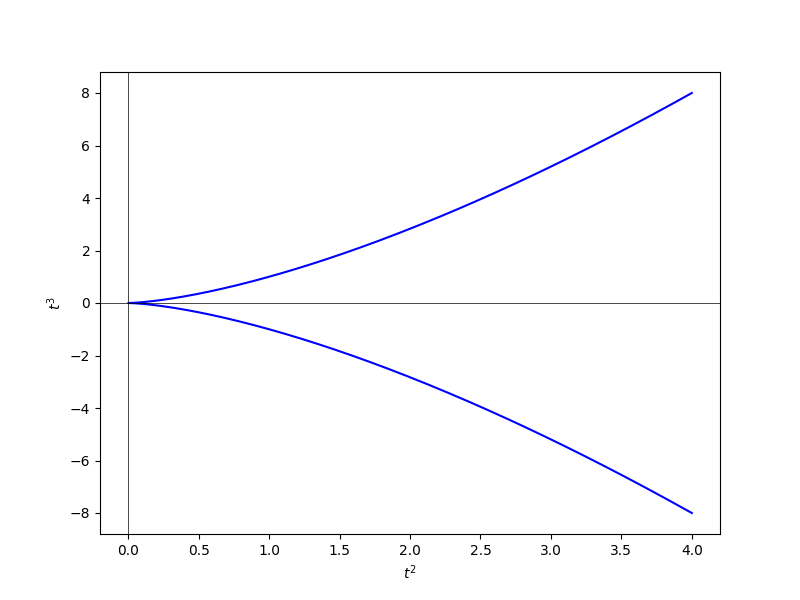
\includegraphics[width=0.5\textwidth]{fig1.png}
			\end{figure}
			
			It is clear that it is a morphism.

			To see if it is continuous first remember that affine space (and also projective space) is equipped with the Zariski topology, whose open sets are complements of algebraic sets (=sets of zeroes of polynomials). But $A=k[x]$ is principal so every algebraic set is the set of zeroes of one polynomial, basically because of this corollary of the Nullstellensatz:
\begin{coro}[[Hart] 1.4]
	There is a one-to-one inclusion-reversing correspondence between algebraic sets in $\mathbb{A}^{n} $ and radical ideals in $k[x_1,\ldots,x_n$ ] (i.e., ideals which are equal to their own radical), given by $Y\mapsto I(Y)$ and $\mathfrak{a}\mapsto Z(\mathfrak{a})$. Furthermore, an algebraic set is irreducible iff its ideal is a prime ideal.
\end{coro}

And $k$ is closed so every polynomial $n$ roots, so algebraic sets are just finite sets.

{\color{magenta}This was seemed relevant at some point…}

\begin{defn}
	The \textit{\textbf{(Krull) dimension}} of a ring $A$ is the supremum of all \textit{\textbf{heights}} of all prime ideals, i.e. the largest proper chain of prime ideals $\mathfrak{p}_0\subset \mathfrak{p}_1\subset\ldots\subset \mathfrak{p}$.
\end{defn}

\begin{prop}[1.7]
	If $Y$ is an affine algebraic set, then the dimension of $Y$ is equal to the dimension of its affine coordinate ring $A(Y)$.
\end{prop}

			We only need to know that closed sets are finite points. This \href{https://math.stackexchange.com/questions/407693/polynomials-are-continuous-with-respect-to-the-zariski-topology}{means} that polynomials are continuous functions with respect to Zariski topology (because preimage of a closed set=finite set of points is closed because it is the root of $p-\alpha$). That makes $\varphi$ continuous.

			Being bicontinuous is the same as being a homeomorphism, which is equivalent to showing that $\varphi$ is open or closed (since we already noted it is bijective). But, finite sets of points are closed sets in the curve (because it is put in affine space---this is not true in general!).

			Finally we show that $\varphi$ is not an isomorphism. Yesterday with Victor we tried to write the inverse map, which should satisfy
\begin{align*}
	 (x,y)&=(\varphi^{-1}(x,y)^2,\varphi^{-1}(x,y)^3)\\
	\implies &\begin{cases}
		\varphi^{-1}(x,y)^2&=x=\frac{x^2}{x^3}=\frac{x^2}{y^2}=\left(\frac{x}{y}\right)^2 \\
		\varphi^{-1}(x,y)^3& =y=\frac{y^2}{y^3}=\frac{x^3}{y^3}=\left(\frac{x}{y}\right)^3
	\end{cases}
\end{align*}
so basically $\varphi^{-1}$ must be $(x,y)\mapsto \frac{x}{y}$ but this is not defined at $y=0$ so I thought well why don't you just put
			\[(x,y)\longmapsto\begin{cases}
				0\qquad &y=0 \\
				\frac{x}{y}\qquad &y\neq 0
			\end{cases}\]
			but then all $(x,0)$ will map to $(0,0)$ under $\varphi\circ \varphi^{-1}$. So what happens is that this map is not well-defined so it is not an isomorphism.

	\item The Frobenius morphism is in fact a ring homomorphism meaining it preserves multiplication and addition. Addition is more \href{https://en.wikipedia.org/wiki/Frobenius_endomorphism#Definition}{interesting}: since $p$ is prime, it divides the numerator and not the denominator of the binomial coefficient $\frac{p!}{k!(p-k)!}$, and this will make that number 0 unless $k=0,n$, which are the first final terms of the binomial expansion  $(a+b)^p$. Therefore we must only show that $\varphi$ has trivial kernel. Now since $k$ is a field, all elements are units, so none of them can actually satisfy $a^p=0$, making $\ker\varphi=0$.

	That $\varphi$ surjective \href{https://en.wikipedia.org/wiki/Perfect_field}{follows} from an equivalence of the field being algebraically closed and thus perfect.

	That $\varphi$ is continuous and bicontinuous follows from the same reasons as the previous question.

	To finish we check that the induced map on coordinates rings is not an isomorphism, since its inverse must be of the form $t\mapsto t^{\frac{1}{p}}$, which is not polynomial.

\end{enumerate}
\end{proof}

\subsection{$\mathbb{P}^n$ minus a hyperplane (Alex)}

\begin{manualexercise}{3.5}[Alex, Sept 17]
	By abuse of language, we will say that a variety \textit{\textbf{is affine}} it is isomorphic to an affine variety. If $H\subseteq \mathbb{P}^n$ is any hypersurface, show that $\mathbb{P}^n-H$ is affine.
\end{manualexercise}

\begin{proof}[Solution]\leavevmode
	Suppose $H=V(f)$ with  $\operatorname{deg}f=d$. Consider the $d$-uple embedding $v_d:\mathbb{P}^n\to \mathbb{P}^N$
\end{proof}


\addcontentsline{toc}{subsection}{Exercise 3.16}
\begin{manualexercise}{3.16}[Products of Quasi-Projective Varieties]
	Use the Segre embedding (Ex. 2.14) to identify $\mathbb{P}^n\times\mathbb{P}^m$ with its image and hence give it a structure of projective variety. Now for any two quasi-projective varieties $X\subseteq\mathbb{P}^n$ and $Y\subseteq\mathbb{P}^m$ consider $X\times Y\subseteq\mathbb{P}^n\times\mathbb{P}^m$.
	\begin{enumerate}[label*=(\alph*)]
		\item Show that $X\times Y$ is a quasi-projective variety.
		\item If $X,Y$ are both projective, show that $X\times Y$ is projective.
		\item Show that $X\times Y$ is a product in the category of varieties.
	\end{enumerate}
\end{manualexercise}

\begin{proof}[Solution]
	content...
\end{proof}

\subsection{Normal varieties}

\begin{manualexercise}{3.17}
	A variety $Y$ is \textit{\textbf{normal}} ar a point $P\in Y$ if $\mathcal{O}_{P}$ is an integrally closed ring. Y is \textit{\textbf{normal}} if it is normal at every point.
\end{manualexercise}

\begin{manualexercise}{3.18, Projective Normal Varieties}
	A projective variety $Y\subseteq \mathbb{P}^n$ is \textit{\textbf{projectively normal}} (with respect to the given embedding) if its homogeneous coordinate ring $S(Y)$ is integrally closed.

	\begin{defn}
		Let $A\subset B$ be a subring (or a morphism $A\to B$) $b\in B$ is \textit{\textbf{integrally closed}} if it is the root of a polynomial in $A[x]$. Here we mean that  $S(Y)$ equals the set of integrally closed elements with respect to its field of fractions.
	\end{defn}

	\begin{enumerate}[label=\alph*.]
		\item If $Y$ is projectively normal, then $Y$ is normal.

		\item There are normal varieties in projective space which are not projectively normal. For
	\end{enumerate}
\end{manualexercise}

\begin{proof}[Solution]\leavevmode
	\begin{enumerate}[label=\alph*.]
		\item $\forall p \in Y$ and prime ideal $\mathfrak{m}_p  \in\operatorname{Spec}(Y)$ we have
			\[S(Y)\subseteq S(Y)_{\mathfrak{m}_p}\subseteq F(Y)\]
			{\color{magenta}How does this conclude?}

		\item 
	\end{enumerate}
\end{proof}

\addcontentsline{toc}{subsection}{5.4}
\begin{manualexercise}{5.4}[Intersection mulitplicity]
	If $X,Y\subseteq \mathbb{A}^{2} $
\end{manualexercise}

\subsection{Sept 10}

\subsubsection{Analitically isomorphic singularities, Arthur}
Two curves $C_1,C_2$ with points $P \in C_1$ and $Q\in C_2$, and $\mathcal{O}_P\supset\mathfrak{m}_P$, $\mathcal{O}_Q\supset\mathfrak{m}_Q$. And
\[C:f=0,\qquad f[x,y]/(f), \quad \mathfrak{m}=(x,y).\]
We define
\[\hat{\mathcal{O}}_p=\lim_{\longleftarrow} \mathcal{O}_P/\mathfrak{m}^n_P\cong k[ [x,y]]/(y)\]

\begin{defn}
	\textit{\textbf{Analitical isomorphism}} is a $k$-isomorphism with $\hat{\mathcal{O}}_P\cong \hat{\mathcal{O}}_Q$.
\end{defn}

\begin{manualexercise}{}
	\begin{enumerate}[label=\alph*.]
		\item An. isomorphic $\implies \mu_{C_1}(D)=\mu_{C_2}(Q)$.
\[f(x,y)=f_r(x,y)+f_{r+1}(x,y)+\ldots+f_n(x,y).\]
\[\mu(p)=r\]

\item Let $f=f_r+f_{r+1}+\ldots\in k[[x,y]]$. Suppose that $f_r=g_s h_t\in k[x,y]$ have no linear factors in common (which means they are coprime). Then there exist $g,h\in k[ [ x,y] ]$ such that
	\[f=gh,\quad g=g_s,\quad h=h_t+\ldots\]

	\item Let $f=f_r+f_{r+1}+\ldots\in k[x,y]$. If
		\[f_r=L_1\cdot L_2\cdot \ldots\cdot L_r\]
		then $P=(0,0)$ is an ordinary $r$-fold. Show that any 2-folds are analitically isomorphic.

		\item Consider the curve $C:f=0,\quad \mu=2$. It is an ordinary 2-fold. Show that
			\[\hat{\mathcal{O}}_P\cong \frac{k[ [ x] ]}{(y^2-x^r)}\]
	\end{enumerate}
\end{manualexercise}

\begin{proof}[Solution]\leavevmode
	\begin{enumerate}[label=\alph*.]
		\item

		\item Suppose they exist and are $g=\sum_{i}g_i$, $h=\sum_{j}h_j$ so that
			\[f=gh=\sum_{d=r}^\infty\sum_{i+j=d}g_ih_j\]
			which means that
			\[f_{r+d}=\sum_{i+j=d}g_ih_j=g_sh_{t+d}+g_{s+d}h_t+\sum_{?}g_ih_j\]
			and
			\[f_{r+1}=g_s h_{t+1}+g_{s+1}h_t\]
			Notice that since $g$ and $h$ don't share linear factors, we may fix the second variable and the resulting polynomials generate $k[t]$, ie.
			\[(g_s(t,1),h_t(t,1))=k[t]\]
			Further computations show that the next term is well defined.

		\item Consider the completion at the origin, $\hat{\mathcal{O}}_P\cong k[[x,y]]/(f)$. We shall try to show that in fact
			\[k[[x,y]]/(f)\overset{\cong }{\longrightarrow}k[ [x,y]]/(f_r)\]
			so consider the map
			\begin{align*}
				x\mapsto x+A(x,y)\qquad \qquad y\mapsto y+B(x,y)
			\end{align*}
			so that
			\[f(x+A(x,y),y+B(x,y))=f_r(x,y).\]
			Using a projective transformation, that makes the tangents be (?), we see that
			\[\hat{\mathcal{O}}_P\cong k[ [x,y]]/(xy)\]

			\begin{claim}[Not true]
		 Any $k$-isomorphism 
		 \[\varphi:\frac{k[ [x,y]]}{(f)}\longrightarrow\frac{k [ [ x,y] ] }{(y)}\]
		 have the form
		 \[x\mapsto x+A(x,y)\quad \quad y\mapsto y+B(x,y)\quad  \text{when } \mu\geq 2\]

		 \item Suppose that
			 \[f(x,y)=y^2A(y)\qquad A(0)\neq 0,\qquad f(x,y)=(y^2+a(x)y+b(x))\cdot u(x,y)\]
			 recall that
			 \begin{thm}[Weierstrass preparation theorem]\leavevmode
				 Let $A$ be a local ring, $k[ [x]]$,  $\mathfrak{m}=(x)$, and $f\in A[ [ y ] ]$. Then
			 \[f=(y^n+k_{r-1}y^{n-1}+\ldots+b_0)\cdot u(y)\]
			 for $u\in A[ [ y] ]^\times $ and $b_i\in\mathfrak{m}$
			 \end{thm}
			 \begin{align*}
			 	f(x,y)& =(y^2+c(x))u(x,y)\\
				\hat{\mathcal{O}}_P&\cong \frac{k[ [x,y]]}{(y^2+c(x))}\\
				c(x)& =x^rV(x),\quad \text{where } V\in k[ [ x]]^\times \\
				V(x)& =1+x+\ldots\\
				\sqrt[r]{1+x} =1+c_1x+\ldots\\
				V(x)& =W(x)^r\\
				x^rV(a)& =(xW)^r\\
				y^2&-x^r.
			\end{align*}
	\end{claim}

	\end{enumerate}
\end{proof}

\subsubsection{Degree and Hilbert polynomial, Bruno}

%\addcontentsline{toc}{subsubsection}{Exercise 7.2}

\begin{defn}
	Let $M$ be a finitely generated graded $S$-module, where $S=k[x_0,\ldots,x_m]$. A \textit{\textbf{Hilbert function}} is
	\begin{align*}
		\varphi: \mathbb{Z} &\longrightarrow M \\
		t &\longmapsto \dim_k(M_t)
	\end{align*}
\end{defn}

\begin{thm}
	There exists a unique polynomial $P_M\in\mathbb{Q}[t]$ such that for all $t\gg 0$, $P_M(t)=\varphi_M(t)$.
\end{thm}

\begin{manualexercise}{7.2}
	Let $Y$ be a variety of dimension $r$ in $\mathbb{P}^n$, with Hilbert polynomial $P_Y$. We define the \textit{\textbf{arithmetic genus}} of $Y$ to be
	\[P_Y(t):=P_{S[Y]}(t)\]
	\[=(-1)^r(P_Y(0)-1)\]
	\begin{enumerate}[label=\alph*.]
		\item  $Y=\mathbb{P}^n$.
		\item $Y\subset \mathbb{P}^n$ plane curve of degree $d$.
		\item $ Y\subset \mathbb{P}^n$ hypersurface of degree $d$.
		\item $Y_a,Y_b\subset \mathbb{P}^3$ of degrees $a$ and $b$, $Y =Y_a\cap Y_b$ complete intersection.
		\item $Y^r\subset \mathbb{P}^n$, $Z^s\subset \mathbb{P}^m$ : $Y\times Z\subset \mathbb{P}^N$. Here
			\[P_{Y\times Z}(t)=P_Y(t)P_Z(t)\]
	\end{enumerate}
\end{manualexercise}

\begin{proof}[Solution]\leavevmode
	\begin{enumerate}[label=\alph*.]
		\item $S[Y]=k[x_0,\ldots,x_n]$, 
		\[\dim (k[x_0,\ldots,x_n]_t)=\binom{n+t}{n}=\frac{(n+1)(n+t-1)\ldots(t+1)}{n!}=\frac{t^n}{n!}+\ldots\]
			so that
			\[P_Y(0)_1\implies P_a(\mathbb{P}^n)=0.\]
	
			\item Now
				\[P_a(Y)=\frac{(d-1)(d-2)}{2}\]
				which follows from c so let's do c.

			\item Suppose $Y=Z(f)$. Then
			\[(f)\hookrightarrow k[x_0,\ldots,x_n]\to k[Y]\]
			\begin{align*}
				(f)& =\{f\varphi:\varphi\in k[x_0,\ldots,x_n]\} \\
				(f)_t&=\binom{n+t-d}{n}\\
			P_Y(t)&=\binom{n+t}{n}-\binom{n+t-d}{n}\\
			P_a(Y)&=(-1)^n\binom{n-d}{n}\\
			&=(-1)^n\frac{(n-d)(n-d-1)\ldots(1-d)}{n!}\\
			&=\frac{(d-1)\ldots(d-n)}{n!}\\
			& =\binom{d-1}{n}
			\end{align*}

			\item Let's first write the formula and then we discuss it
				\begin{align*}P(t)&=\binom{3+t}{t}-\binom{3+t-a}{t}-\binom{3+t-b}{t}+\binom{3+t-a-b}{3}\\
					&=(ab)t+P_Y(0)
					\end{align*}
					\begin{align*}
						P_Y(0)&=1-f(a)-f(b)+f(a+b)\\
						P_a(Y)&=f(a)+f(b)-f(a+b)
					\end{align*}
					Considering multiplication by $f_b$ as map
					\[\frac{k[\mathbb{P}^3]}{(f_a)}\overset{f_b}{\longrightarrow}\frac{k[\mathbb{P}^3]}{(f_a)}\]
					so we get
					\[\begin{tikzcd}
						0\arrow[r]&\frac{k[\mathbb{P}^3]}{(f_a)}\arrow[r]&\frac{k[\mathbb{P}^3]}{(f_a)}\arrow[r]&\frac{k[\mathbb{P}^3]}{(f_a,f_b)}\arrow[r]&0
					\end{tikzcd}\]
					but we need to consider the map $[-b]$ to stop the grading from moving up from one arrow to another. Then we get
					\[P_Y=P_{Y_a}(t)-P_{Y_a}(t-b)\]
					so
					\[P_A-P_B+P_C=0.\]

	\item O problema est\'a em ver se
		\[K[Y\times Z]_d\overset{?}{\cong}k[Y]_d \otimes_k k[Z]_d\]
	Da\'i o Hilbert polynomial \'e o produto dos Hilbert polynomials e t\'a.
	\end{enumerate}
\end{proof}

\subsection{Degree of Veronese and Segre embeddings, Alex, Sept 13}

%\addcontentsline{toc}{subsection}{Exercise 7.1}
\begin{manualexercise}{7.1}\leavevmode 
	\begin{enumerate}[label=\alph*.]
		\item Find the degree of the 2-uple embedding of $\mathbb{P}^n$ in $\mathbb{P}^N$.

		\item Find the degree of the Segre embedding of $\mathbb{P}^r\times \mathbb{P}^s$ in $\mathbb{P}^N$.
	\end{enumerate}
\end{manualexercise}

\begin{proof}[Solution]\leavevmode
\begin{enumerate}[label=\alph*.]
	\item Recall that the degree of a map the coefficient of greatest degree of the Hilbert polynomial times the degree factorial, i.e. if the Hilbert polynomial is
	\[P_{X}(z)=a_nz^n+\ldots+a_0,\]
	the degree of $X$ is
	\[a_nn!\]
	(So remember that the Hilbert polynomial is the unique polynomial in $\mathbb{Q}[t]$ that equals the Hilbert function (the Hilbert functions at $n$ is just the dimension of the degree-$n$ component of $S[X]=\bigoplus_{n} S_n $, so homogeneous polynomials of degree $n$) for sufficiently large numbers.)

	\begin{claim}
		\[S(X)_m \cong k[x_0,\ldots,x_n]_{md}\]
		where $d$ is the $d$ in the $d$-uple embedding.
	\end{claim}
	If we show this, we can see that
	\[P_{x}(m)=\binom{md+n}{n}=\prod_{i=1}^n\frac{(md+i)?}{n!}=\frac{d^nm^n}{n!}+\text{lower order terms}  \]
	Now the pullback map is
	\[\frac{k[x_0,x_1,\ldots,x_N}{I(X)}\overset{\cong }{\longrightarrow}?k[x_0,x_1,\ldots,x_n]\]

	\item 
	
	\end{enumerate}

\end{proof}

\subsection{Sept 20}
\subsubsection{Sergey}

You can find this $\operatorname{Sec}^k$ on a book by Harris, name?

There is an exercise from last class:
%\addcontentsline{toc}{subsubsubsection}{Exercise from Sergey, Sept 17}
\begin{manualexercise}{from Sergey, Sept 17}
	Compute $\operatorname{Sec}^k $ of $\operatorname{Segre}(a,b)$.
\end{manualexercise}

For today:
%\addcontentsline{toc}{subsubsubsection}{Exercise}
\begin{manualexercise}{(Sergey, Sept 20)}\leavevmode 
	\begin{enumerate}[label=\alph*.]
		\item Compute $\dim \operatorname{Gr}(k,N)$. You can use that $\operatorname{GL}(N)$ acts transitively.
		\item $\dim \operatorname{Sec}^k\operatorname{Gr}(N,2)$. \textbf{Hint:} Use linear algebra: $\Sigma_{0,n}=\operatorname{Cone}(\mathcal{v}_{n}\mathbb{P}^1$, $\mathbb{F}_{n}$ Hinzbruch surfaces. Rational Ruled Normal Surfaces (see below for definition of scroll ie. $\Sigma_{0,n}$.
	\end{enumerate}
\end{manualexercise}

\begin{defn}
	The \textit{\textbf{Segre embedding }} is 
	 \begin{align*}
		 \mathbb{P}(U)\times \mathbb{P}(V)&\hookrightarrow \mathbb{P}(U\otimes W)  \\
		 ([u],[v]) &\longmapsto [u\otimes v]
	\end{align*}
	Now take $X\subset \mathbb{P}(W)$. Then
	\[\operatorname{Sec}^k(X)=\overline{Z}\]
	where
	\[Z=\{[w]:\exists p_1,\ldots,p_k\in X\hookrightarrow \mathbb{P}(W)\} =\bigcup_{p_1,\ldots,p_k\in X}\left<p_1,\ldots,p_k\right>  \]
	where $p_i=[v_i]$ and $w=\sum_{i}v_i$.
\end{defn}

\begin{defn}[Scroll]
	I have a variety $X$ and two linear systems:
	\[\begin{tikzcd}
	&X\arrow[dl,"\varphi",hook,swap]\arrow[dr,"\psi",hook]\\
	\mathbb{P}(U)&&\mathbb{P}(V)
	\end{tikzcd}\]
	Then the \textit{\textbf{scroll}} is
	\[\mathbb{P}(U\oplus V)\supset\Sigma_{\varphi,\psi}=\{[u\oplus v]:[u]\in\varphi(X),[v]\in\psi(X)\}\]
	\textbf{Exercise:} Show this is a projective variety.

	So the scroll is a union of projective lines. It is called scroll because lines in one direction survive (in a drawing, they are all parallel) but the other lines are curved (so it looks like a scroll).
\end{defn}

%\addcontentsline{toc}{subsubsubsection}{Exercise about scroll}
\begin{manualexercise}{about scroll}
	As abstract varieties, $\Sigma_{a,b}$ is isomorphic to $\Sigma_{a'b'}$ iff $b-a=b'-b'=n$ and either  $a=a'=0$ or  $a>0, a'>0$.
\end{manualexercise}

\subsubsection{Alex}
%\addcontentsline{toc}{subsubsubsection}{Exercise 6.3, Elliptic curve is not rational}
\begin{manualexercise}{6.3, Elliptic curve is not rational}
	Let  $Y$ be the curve $y^2=x^3-x$ in $\mathbb{A}^2$, and assume that the characteristic of the base field $k$ is not 2. In this exercise we will show that $Y$ is not a rational curve, and hence $K(Y)$ is not a pure trascendental extension of $k$.
\begin{enumerate}[label=\alph*.]
	\item Show that $Y$ is nonsingular, and deduce that $A=A(Y)\cong \frac{k[x,y]}{(y^2-x^3+x}$.
	\item Let $k[x]$ be the subring of …
\end{enumerate}
\end{manualexercise}

%\addcontentsline{toc}{subsubsection}{Exercise 6.2}
\begin{manualexercise}{6.2}
Let
	\[Y=V(y^2-x^3+x\subset \mathbb{A}^2\]
	be an elliptic curve. Show it is not rational.
\end{manualexercise}

\begin{defn}
	A curve $C$ is \textit{\textbf{rational}} if $C$ is birationally equivalent to $\mathbb{P}^1$
\end{defn}

\paragraph{Fact} If $C$ is a nonsingular rational but not isomorphic to $\mathbb{P}^1$, then $A(C)$ is a UFD.

\begin{enumerate}[label=\textbf{Step \arabic*}]
	\item $Y$ is nonsingular. Looks like we can just differentiate here and find that the zero locus of the derivatives is not in $C$.
\begin{defn}[Tangent space]
	Consider the local ring at the point and its maximal ideal. So $\mathfrak{m}_{p}/\mathfrak{m}^2_p$ is the \textit{\textbf{cotangent space}}. Then the  \textit{\textbf{tangent space}} is the dual  $\left(\frac{\mathfrak{m}}{\mathfrak{m}^2}\right)^*$. A point is \textit{\textbf{singular}} if the tangent space has more dimension than it should.
\end{defn}

\paragraph{Interpretation} Functions in $\mathfrak{m}_p$ are those which vanish at $p$. A function in $\mathfrak{m}_{p}$ is $\sum_{i}f_ig_i$ so its differential is $ d \left( \sum_{i}f_ig_i \right) =\sum_{i}f_idg_i+\sum_{i}g_ifd_i$ which you want to mod out because it is zero at $p$ because both $f_{i}$ and $g_{i}$.

\begin{remark}
	For $X,Y\subset Z$, $T_pX,T_pY\subset T_pZ$
	\[T_p(X\cap Y)=T_pX\cap T_pY\]
\end{remark}

\item 
	\begin{thm}[5.1]\leavevmode
		$Y\subseteq \mathbb{A}^n$ affine variety and $P\in Y$. Then $Y$ is nonsingular at $P \iff $ local ring $\mathcal{O}_{P,Y}$ is a regular local ring
	\end{thm}
	\begin{thm}[6.2A]\leavevmode
		$A$ noetherian local domain of sdimension one with maximal ideal $\mathfrak{m}$. Then the following are equivalent
		\begin{enumerate}[label=(\roman*)]
			\item $A$ is a regular local ring.
			\item $A$ is integrally closed (over the fraction field).
		\end{enumerate}
	\end{thm}
	In other words, normality in dimension 1 is the same as normality.

	\item Here's the \textit{\textbf{hyperelliptic involution}}
		\begin{align*}
			\sigma: k[Y] &\longrightarrow K[Y] \\
		x &\longmapsto x\\
		y&\longmapsto-y
	\end{align*}
	and then there's the \textit{\textbf{norm}}
	\begin{align*}
		N: K[Y] &\longrightarrow K[Y] \\
		a&\longmapsto a\sigma(a)
	\end{align*}
	Notice that
	\[N(1)=1\qquad N(a,b)=N(a)N(b)\]
	\textbf{Explanation:} we are killing $y$, so the norm takes us to a simpler space which is $Y/\sigma$.

This means $X$ is irreducible, $Y$ is irreducible. Then a discussion on the invertibility of the norm, units on these rings…
\end{enumerate}

 \subsubsection{Bruno}

\begin{manualexercise}{5.10}
$X$ afine variety and $p\in X$.
\begin{enumerate}[label=\alph*.]
	\item $\dim T_pX\geq \dim X$, $\dim T_pX\iff p$ is nonsingular. Here $\dim X=\dim \mathcal{O}_{P,X}$ which is just the Krull dimension, so maximum height of chain of prime ideals.
	\item Define the tangent map.

	\item Project the parabola $x=y^2$ in $\mathbb{A}^2$ to the  $x$ axis and compute its derivative at 0.
		\end{enumerate}
\end{manualexercise}

\begin{proof}[Solution]\leavevmode
\begin{itemize}
\item $\dim T_pX=\dim \mathfrak{m}_p/\mathfrak{m}^2_p$, \textit{ as a vector space!} . Now that inequality is a result in homological algebra:
	\begin{thm}
		$A$ noetherian local domain and $ \mathfrak{m}$ maximal ideal then the dimension of the quotient of ideals as a vector space is greater or equal to the dimension of $A$ as a ring.
	\end{thm}
	\item 
		\begin{defn}
			$X\overset{\varphi}{\longrightarrow}Y$, $\varphi^*:\mathcal{O}_Y\to \mathcal{O}_X$ which is precomposition. Then since $\varphi(p)=q$ we see that $\varphi^*(\mathfrak{m}_q)\subset \mathfrak{m}_p\implies \varphi^* (\mathfrak{m}^k_q)\subset \mathfrak{m}^k_{p}$. And then take quotient by $\mathfrak{m}_{p}$ and $\mathfrak{m}^2_{q}$. These local rings are the functions that vanish at the point. Also they are localization of polynomials by maximal ideal.
		\end{defn}
\item
	 \begin{claim}
		 $(T\varphi)_0=0$
	\end{claim}
	look at the pullback
	\begin{align*}
		\varphi^*: k[\mathbb{A}^1] &\longrightarrow k[Z]=k[x,y]/(x-y^2) \\
		t &\longmapsto x
	\end{align*}
	which follows from definition.
	
	Then
	\[\varphi^*(\mathfrak{m}_{0})\subset \mathfrak{m}^2_{(0,0)}\implies \varphi^* :\mathfrak{m}_0/\mathfrak{m}_0^2\to \mathfrak{m}_{0,0}/\mathfrak{m}_{0,0}^2\]
	is zero because
	\[\varphi^* (t)=x=y^2,\qquad y\in\mathfrak{m}_{(0,0)}\]
	
\end{itemize}\end{proof}




%\addcontentsline{toc}{subsection}{Exercise Sergey}
\begin{manualexercise}{Sergey}
	Is the variety $\sum_{i=0}^sx_i^3=0$ rational in $\mathbb{P}^5$.
\end{manualexercise}

%\subsection{Blowing up curve singularities (Dani)}




\section{[Ot] Chapter I: Varieties}

A friend from Cabo Frio just recommended me to have a look at \href{https://www.uio.no/studier/emner/matnat/math/MAT4215/data/masteragbook.pdf}{Ottem\&Ellinsburg, Introduction to Schemes}. Here are some exercises I liked from Chapter 1: Varieties.

\addcontentsline{toc}{subsection}{Exercise 1.5.12}
\begin{manualexercise}{1.5.12}[The diagonal]
	Let $X$ be an affine variety and consider the map
	\begin{align*}
		\Delta: X &\longrightarrow X\times X \\
		x &\longmapsto (x,x)
	\end{align*}
	\begin{enumerate}[label=\alph*.]
		\item Show that $\Delta$ is a polynomial map.
		\item Let $X=\mathbb{A}^{n}(k)$…
		\item …gives an isomorphism $X\to \Delta(X)$. Hint…
	\end{enumerate}
\end{manualexercise}

\addcontentsline{toc}{subsection}{Exercise 1.5.15}
\begin{manualexercise}{1.5.15}
{\color{magenta}Some Lie groups that are algebraic sets}
\end{manualexercise}

\addcontentsline{toc}{subsection}{Exercise 1.5.28}
\begin{manualexercise}{1.5.28}
	Show that the image of the map
	\begin{align*}
		\phi: \mathbb{A}^{1}(k) &\longrightarrow \mathbb{A}^{3}(k) \\
		t &\longmapsto (t^{2},t^{3},t^{6})
	\end{align*}
	is given by $V(x^{3}-y^{2},z-x^{3})$. Show that $\phi$ is bijective. Is $\phi$ an isomorphism of affine varieties.
\end{manualexercise}

\addcontentsline{toc}{subsection}{Exercise 1.5.29}
\begin{manualexercise}{1.5.29}
	Show that the image of the map
	\begin{align*}
		\phi: \mathbb{A}^{1}(k) &\longrightarrow \mathbb{A}^{3}(k) \\
		t &\longmapsto (t^{3},t^{4},t^{5})
	\end{align*}
	is given by $V(x^{4}-y^{3},z^{3}-x^{5},y^{5}-z^{4})$. Show that $\phi$ is bijective. Is $\phi$ an isomorphism of affine varieties.
\end{manualexercise}

\addcontentsline{toc}{subsection}{Exercise 1.5.31}
\begin{manualexercise}{1.5.31}
	Show that the image of the map
	\begin{align*}
		\phi: \mathbb{P}^{1}(k) &\longrightarrow \mathbb{P}^{2}(k) \\
		(x_0:x_1( &\longmapsto (x_0^{2},x_0x_1,x_1^{2})
	\end{align*}
	is given by $V(y_1^{2}-y_0y_2)$. Show that $\phi$ is an isomorphism of projective varieties. Deduce that any projective conic is isomorphic to $\mathbb{P}^{1}(k)$.
\end{manualexercise}

\section{Chapter  II}

\subsection{September 24}

\subsubsection{Generically finite morphisms (Arthur)}

\begin{manualexercise}{2.37}
	
\end{manualexercise}

\begin{proof}[Solution]\leavevmode
	\textbf{First part.}
We will show the hint: the field extension $K(X) \subseteq K(Y)$ is finite.

Let $V = \operatorname{Spec} A \subseteq Y$ and $U = \operatorname{Spec} B \subseteq f^{-1}(V) \subseteq X$ be affine open subsets.
Write $C$ for the coordinate ring of $f^{-1}(\eta) \cap U$.

Since $f$ is of finite type, $C$ is finitely generated as a $K(Y)$-algebra.
Explain more. % B is fin gen over A and C is a quotient and localization of B
By Noether's normalization lemma, there exist $y_1, \ldots, y_d \in C$ such that $C$ is finite over $K(Y)[y_1,\ldots,y_d]$, where $d = \dim C$.
But $\dim C = \dim (f^{-1}(\eta) \cap U) = 0$ because $f^{-1}(\eta) \cap U$ is a finite set.
Hence $C$ is finite over $K(Y)$, i.e., $C$ is a finite $K(Y)$-vector space.
In particular, $K(X) \subseteq C$ is finite over $K(Y)$.

\textbf{Second part.}
We will show that there is an open affine $V \subseteq Y$ and an affine open cover $\{U_i\}$ of $f^{-1}(V)$ such that each restriction $U_i \to V$ is finite.

Let $V=\operatorname{Spec} A \subseteq Y$ be an open affine.
Since $f$ is of finite type, there is a finite affine open cover $U_i = \operatorname{Spec} B_i$ of $f^{-1}(V)$ such that $B_i$ is an $A$-algebra of finite type. Let $\{x_{ij}\}$ be a set of generators for $B_i$.
Now $B_i \subseteq K(X)$ and $K(X)$ is a finite $K(Y)$-module, so each $x_{ij}$ is integral over $K(Y)$, i.e., there are polynomials $P_{ij}(T) \in K(Y)[T]$ such that $P_{ij}(x_{ij}) = 0$.

There a is distinguished open subset $V_g \subseteq V$ such that $P_{ij}(T) \in \mathcal{O}_Y(V')[T]$ for all $i,j$.
Replace $U_i$ by $(U_i)_g$ and $V$ by $V_g$. Then $B_i$ is finite over $A$ because it is finitely generated by integral elements.
Hence $f : U_i \to V$ is a finite morphism ($U_i$ and $V$ are affine) for all $i$.

\textbf{Third part.}
Find an affine $V \subseteq Y$ such that $f^{-1}(V)$ is affine.

Now let $U \subseteq \bigcap_i U_i$ be an affine open.
Then $U \subseteq f^{-1}(V)$ and $f : U \to V$ is affine. We will show that we can choose an affine open $V' \subseteq V$ such that $f^{-1}(V') \subset U$. Then we will have $f : f^{-1}(V') \to V'$ affine, concluding the exercise.

To do this, let $Z = f^{-1}(V) \setminus U$.
If $\eta \in \overline{f(Z)}$ then actually $\eta \in f(Z)$ because it is the generic point of $V$.
Looking at the affine $U_i = \operatorname{Spec} B_i$, we see that any $z \in U_i \cap Z$ such that $\eta = f(z)$ corresponds to a prime $\mathfrak{p} \subseteq B_i$ such that $\mathfrak{p} \cap A = (0)$. Since $\mathfrak{p}$ is above the prime $(0) \subseteq A$, the following theorem tells us that $\mathfrak{p} = (0)$:

\begin{thm}[Cohen]\leavevmode
	
\end{thm}

But $(0) \in U$ and $Z \cap U = \varnothing$. Hence $\eta \not \in \overline{f(Z)}$.
Therefore there is some neighborhood $V'$ of $\eta$ such that $V' \cap f(Z) = \varnothing$, which is what we had to show.

Alternatively, let $Z = f^{-1}(V) \setminus U_1$. The same theorem shows that $f(Z)$ is closed. Since $U_i \to V$ is finite for all $i$, we have $\dim f^{-1}(V) = \dim V$. Moreover
\begin{equation*}
	\dim V = \dim f^{-1}(V) > \dim Z \geq \dim f(Z),
\end{equation*}
so $f(Z) \ne V$ and there is an open affine $V'$ such that $V' \cap f(Z) = \varnothing$.
\end{proof}

\subsubsection{Closed subschemes of $\operatorname{Proj}(S)$ (Dani)}

\begin{remark}[Görtz \& Wedhorn, p. 375]
	If $\varphi:A\to B$ is a homomorphism of graded $R$-algebras, the inverse image of a relevant prime ideal (not containing the homogeneous ideal of positive degree groups $\bigoplus_{d\geq 1} S_d $) of $B$ may not be a relevant prime ideal of $A$. Thus $\operatorname{Proj}(A)$ is not func torial in $A$ with respect to arbitrary homomorphisms of graded $R$-algebras. But there is a unique morphism of $R$-schemes
	\[\operatorname{Proj}\varphi:G(\varphi)\longrightarrow \operatorname{Proj}A,\]
	where $G(\varphi )\subseteq \operatorname{Proj}(B)$ is the open subscheme
	\[G(\varphi )=\mathfrak{q}\in\operatorname{Proj}(B):\varphi^{-1}(\mathfrak{q})\not\supset A_+\}\]
such that …
\end{remark}

\begin{manualexercise}{2.14}\leavevmode 
	\begin{enumerate}
		\item[(b)] Let $\varphi:S\to T$ be agraded homomorphism of graded rings (preserving degrees). Let $U=\{\mathfrak{p}\in\operatorname{Proj}(T):\mathfrak{p}\not\supseteq\varphi(S_+)\}$. Show that $U$ is an open subset of $\operatorname{Proj}(T)$ and show that $\varphi$ determines a natural morphism $f: U\to \operatorname{Proj}(S)$.
	
		\item[(c)] The morphism $f$ can be an isomorphism even quen $\varphi$ is not. For example, suppose that $\varphi_d:S_d\to T_d$ is an isomorphism for all $d\geq d_0$, where $d_0$ is an integer. Then show that $U=\operatorname{Proj}T$ and the induced morphism $f:\operatorname{Proj}T\to  \operatorname{Proj}S$ is an isomorphism.
	\end{enumerate}
\end{manualexercise}

So basically the following exercise is about studying a case when this induced morphism behaves nicely, namely when $\varphi$ is surjective.

\begin{manualexercise}{3.12}\leavevmode 
	\begin{enumerate}[label=\alph*.]
		\item Let $\varphi:S \to T$ be a surjective homomorphism of graded rings, preserving degrees. Show that the open set $U$ from exercise 2.14 is equal to $\operatorname{Proj}T$ and the morphism $f$ is a closed immersion.

		\item If $I\subseteq S$ is a homogeneous ideal, take $T=S/I$ and let  $Y$ be the closed subsceme of $\operatorname{Proj}S$ defined as the image of the closed immersion $\operatorname{Proj}(S/I)\to \operatorname{Proj}S$. Show that different homogeneous ideals can give rise to the same closed subscheme.
	\end{enumerate}
\end{manualexercise}

\begin{defn}[3.41 Gortz]
	A morphism $i:Z\to X$ of schemes is called a \textit{\textbf{closed immersion}} if the underlying continuous map is a homeomorphism between $Z$ and a closed subset of $X$ and the sheaf homomorphism $i^\flat:\mathcal{O}_X\longrightarrow i_*\mathcal{O}_Z$ is surjective.
\end{defn}

\begin{proof}[Solution]\leavevmode
	\begin{enumerate}[label=\alph*.]
	\item The fact that $U=\operatorname{Proj}T$ is immediate from definition and sujectivity since  $\varphi(S_+)=T_+$.  The induced map is
		\begin{align*}
			f: U= \operatorname{Proj}T &\longrightarrow \operatorname{Proj}S \\
			\mathfrak{p} &\longmapsto \varphi^{-1}(\mathfrak{p})
		\end{align*}
	Now let's see that $f$ is a closed immersion. 

	\textbf{$f$ is injective.} Follows from surjectivity: if $\mathfrak{p},\mathfrak{q}\in\operatorname{Proj}T$ are such that $\varphi^{-1}(\mathfrak{p})=\varphi^{-1}(\mathfrak{q})$, then $\varphi(\varphi^{-1}(\mathfrak{p}))=\mathfrak{p}=\mathfrak{q}=\varphi(\varphi^{-1}(\mathfrak{q}))$.

	\textbf{$f(\operatorname{Proj}T)$ is closed} We claim that 
	\begin{align*}f(\operatorname{Proj}T)&=V\left(\bigcap_{\mathfrak{p}\in\operatorname{Proj}(T)}\varphi^{-1}(\mathfrak{p})\right)\\
		&=\left\{ \mathfrak{q}\in\operatorname{Proj}S:\mathfrak{q}\supseteq\bigcap_{p\in\operatorname{Proj}T} \varphi^{-1}(\mathfrak{p}) \right\} 
		\end{align*}
The contention $\subseteq$ is clear since  $\varphi^{-1}(\mathfrak{q})\in f(\operatorname{Proj}T)\implies \varphi^{-1}(\mathfrak{q})\supseteq\bigcap_{q\in\operatorname{Proj}T} \varphi^{-1}(\mathfrak{p})$.

For $\supseteq$ we want to see that $\mathfrak{q}=\varphi^{-1}(\varphi(\mathfrak{q}))$. Suppose that there exists $x\in\varphi^{-1}(\varphi(\mathfrak{q}))\setminus \mathfrak{q}$. Then there exists $y\in\mathfrak{q}$ such that  $\varphi (x)=\varphi (y)\implies \varphi (x-y)=0$. But $0=(x-y)\subset \bigcap_{\mathfrak{p}\in\operatorname{Proj}T} \varphi(\mathfrak{p})$, meaning $x-y\in\mathfrak{q}$, but that is not possible since $ x\not\in\mathfrak{q}$.

	\textbf{$f$ is a homeomorphism} It preserves inclusions of ideals?

\textbf{Induced map on stalks is surjective} What is going on?

\begin{remark}[Gortz, p. 57]
A morphism $(f,f ^\flat):X\to Y$ of ringed spaces induces morphisms on the stalks as follows. Let $x\in X$. Let $f^\sharp:f^{-1}\mathcal{O}_Y\to  \mathcal{O}_X$ be the morphism corresponding to $f ^\flat$ by adjointness. Using the identification $(f^{-1}\mathcal{O}_Y)_x=\mathcal{O}_{Y,f(x)}$ established in $(2.8.2)$ we get
\[f^\sharp _x:\mathcal{O}_{Y,f(x)}\longrightarrow \mathcal{O}_{X,x}.\]
\end{remark}
So I'm not really sure how this is defined but we are looking at a map
\[f^\sharp _x:\mathcal{O}_{f(\operatorname{Proj}T)}\longrightarrow \mathcal{O}_{\operatorname{Proj}S}\]

	Ah! Now I see:
	\begin{prop}[2.5]\leavevmode 
	\begin{enumerate}[label=\alph*.]
		\item For any $\mathfrak{p}\in\operatorname{Proj}S$, the stalk $\mathcal{O}_\mathfrak{p}$ is isomorphic to the local sing $S_{(\mathfrak{p})}$.
	\end{enumerate}
\end{prop}
So in fact we have some map $f^\sharp_\mathfrak{p}:S_{(\varphi^{-1}(\mathfrak{p}))}\longrightarrow T_{(\mathfrak{p})}$. I don't really know how this is defined, but in a broad sense we know this is a map induced by $\varphi$, which was surjective, acting on the localizations of $S$ and $T$, which are really $S$ and $T$ made larger by adding some fractions.

\item Let $d_0$ be an integer and define $I'=\bigoplus_{d\geq d_0}I_d$. Basically this is just exercise 2.14(c). We just notice that $I'$ just  $I$ taking away the first $d_0$ degrees, so we have a projection map
	\[\varphi:S/I'\to S/I\]
	which is just the identity after degree $d_0$. That is the hypothesis of exercise 2.14(c), which yield an isomorphism $\operatorname{Proj}(S/I)\cong \operatorname{Proj}(S/I')$. And that clearly means that the induced subschemes of $\operatorname{Proj}S$ are isomorphic.
	
	\end{enumerate}
\end{proof}


\section{Chapter III}

\subsection{Injective resolutions, derived functors and cohomology (once and for all?)}
\begin{defn}
	(\href{https://en.wikipedia.org/wiki/Injective_object#:~:text=9%20References-,Definition,can%20be%20extended%20to%20Y%20.}{wiki}) An object $Q$ is \textit{\textbf{injective}} if, given a monomorphism $f:X\to Y$, any $g:X\to Q$ can be extended to $Y$.
\[\begin{tikzcd}
X\arrow[r,"f",hook]\arrow[d,"g",swap]&Y\arrow[dl,"h",dashed]\\
Q
\end{tikzcd}\]
\end{defn}

(\href{https://en.wikipedia.org/wiki/Derived_functor#Construction_and_first_properties}{wiki}) The crucial assumption we need to make about our abelian category (=morphisms and objects can be added and kernels and cokernels exist and have desiarable properties) is that it has  \textit{\textbf{enough injectives}}, meaning that for every object $A$ in $\mathbf{A}$ there exists a monomorphism $A\to I$ where $I$ is an injective object in $\mathbf{A}$.

The right derived functors of the covariant left-exact functor $F:A\to B$ are then defined as follows. Start with an object $X$ of $\mathbf{A}$. Because there are enough injectives, we can construct a long exact sequence of the form
\[\begin{tikzcd}[column sep=small]
	0\arrow[r]&X\arrow[r]&I^0\arrow[r]&I^1\arrow[r]&I^2\arrow[r]&\cdots
\end{tikzcd}\]
where $I^i$ are injective. (This is known as an \textit{\textbf{injective resolution}} of $X$). Applying the functor $F$ to this sequence, and choppingng off the first term, we obtain the chain complex
\[\begin{tikzcd}[column sep=small]
	0\arrow[r]&F(I^0)\arrow[r]&F(I^1)\arrow[r]&F(I^2)\arrow[r]&\cdots
\end{tikzcd}\]
This is in general not an exact sequence anymore. But we can compute its cohomology at the $i$-th spot (the kernel of the map from $F(I^i)$ modulo the image of the map to $F(I^i))$; we call the result $R^iF(X)$.

Of course various things have to be checked: the result does not depend on the given injective resolution of $X$, and any morphism $X\to Y$ naturally yields a morphism $R^iF(X)\to R^iF(Y)$ so that we indeed obtain a functor. Note that left exactness means that
\[\begin{tikzcd}
	0\arrow[r]&F(X)\arrow[r]&F(I^0)\arrow[r]&F(I^1)\arrow[r]&0
\end{tikzcd}\]
is exact, so $R^0F(X)=F(X)$, so we only get something interesting for $i>0$. (In Hartshorn Thm 1.1A: $F\cong R^0F$.)

\paragraph{Explanation} A \textit{\textbf{derived functor}} of a given functor maps an object to the $i$-th cohomology of the image of an injective resolution of the object.

The above-mentioned (where?) property of turning short exact sequences into long exact sequences is a consequence of the snake lemma. In Hartshorne Thm 1.1A: For each short exact sequence
\[\begin{tikzcd}
	0\arrow[r]&A'\arrow[r]&A\arrow[r]&A''\arrow[r]&0
\end{tikzcd}\]
and for each $i\geq 0$ there is a natural morphism $\delta^i:R^iF(A'')\to R^{i+1}F(A')$ such that we obtain a long exact sequence
\[\begin{tikzcd}[column sep=small]
	\cdots\arrow[r]&R^iF(A')\arrow[r]&R^iF(A)\arrow[r]&R^iF(A'')\arrow[r,"\delta^i"]&R^{i+1}F(A')\arrow[r]&R^{i+1}F(A)\arrow[r]&\cdots
\end{tikzcd}\]


\begin{prop}[2.1A,  Cateogory of $A$-modules has enough injectives]
	If $A$ is a ring, then every $A$-module is isomorphic to a sub-module of injective $A$-module.
\end{prop}

\begin{proof}
	Hartshorne cites other resources.
\end{proof}

\begin{prop}
	Let  $(X,\mathcal{O}_X)$ be a ringed space. Then the category $\mathfrak{Mod}(X)$ of sheaves of $\mathcal{O}_X$-modules has enough injectives.
\end{prop}

\begin{coro}
	If $X$ is any topological space, then the category $\mathfrak{Ab}(X)$ of sheaves of abelian groups on $X$ has enough injectives.
\end{coro}

\begin{proof}
	Just because abelian groups are $\mathbb{Z}$-modules so it's just a particular case of the last theorem.
\end{proof}

\begin{defn}
	The \textit{\textbf{cohomology functors}} of a topological space $X$ are the derived functors of the global section functor $\Gamma(X,\cdot)$. {\color{magenta}(What is this global sections functor for any topological space?)} For any sheaf $\mathcal{F}$, the groups $H^{i}(X,\mathcal{F})$ are the \textit{\textbf{cohomology groups}} of  $\mathcal{F}$.
\end{defn}

\begin{remark}
	This is equivalent to sheaf cohomology construction via \v Cech cohomology.
\end{remark}

\section{Chapter IV}

\addcontentsline{toc}{subsection}{Exercise 1.2}
\begin{manualexercise}{1.2}[I like this one]
	Again let $X$ be a curve, and let $P_1,\ldots,P_r$ be points. Then there is a rational  function $f\in K(X)$ having poles (of some order) at each of the $P_i$ and regular  elsewhere.  
\end{manualexercise}

\addcontentsline{toc}{subsection}{Exercise 1.7}
\begin{manualexercise}{1.7}[no one]
	A curve $X$ is called \textit{\textbf{hyperelliptic}}…
\end{manualexercise}

\addcontentsline{toc}{subsection}{Exercise 1.8}
\begin{manualexercise}{1.8}[Alex]
	Very useful to know, I think this is done in that book by Bosch of modules,
\end{manualexercise}

\addcontentsline{toc}{subsection}{Exercise 1.9}
\begin{manualexercise}{1.9}[Victor]
	Riemann-Roch for singular curves.
\end{manualexercise}

\addcontentsline{toc}{subsection}{Exercise 2.3(h)}
\begin{manualexercise}{2.3(h)}
	28 bitangents. Remind Sergey.
\end{manualexercise}

\addcontentsline{toc}{subsection}{Exercise 2.5}
\begin{manualexercise}{2.5}
	Prove the theorem of Hurwitz that a curve $X$ of genus $g\geq 2$ over a field of characteristic 0 has at most $84(g-1)$.
\end{manualexercise}

\addcontentsline{toc}{subsection}{Exercise 3.1}
\begin{manualexercise}{3.1}
	If X is a curve of genus 2, show that a divisor D is very ample $\iff \operatorname{deg} D \geq 5$.  This strengthens (3,3.4).
\end{manualexercise}

\addcontentsline{toc}{subsection}{Exercise 3.12}
\begin{manualexercise}{3.12}
	For each value of $d = 2,3,4,5$ and $r$ satisfying $0\leq r\leq \frac{1}{2}(d-1)(d-2)$, show  that there exists an irreducible plane curve of degree d with r nodes and no other  singularities.
\end{manualexercise}

\addcontentsline{toc}{subsection}{Exercise 4.10}
\begin{manualexercise}{4.10}
	If $X$ is an elliptic curve (Sergey: for abelian varieties is also true), show that there is an exact sequence… Picard groups.
\end{manualexercise}

\addcontentsline{toc}{subsection}{Exercise 5.3}
\begin{manualexercise}{5.3}
	Moduli of Curves of Genus 4. The hyperelliptic curves of genus 4 form an irreducible family of dimension 7. The nonhyperelliptic ones form an irreducible  family of dimension 9. The subset of those having only one $g_3^{1}$ is an irreducible  family of dimension 8. [Hint: Use (5.2.2) to count how many complete intersections $Q\cap F_3$ there are.]  
\end{manualexercise}

%\addcontentsline{toc}{subsection}{Exercise 6.2}
\begin{manualexercise}{6.2}
	A rational curve of degree 5 in $\mathbb{P}^{3}$ is always contained in a cubic surface, but there  are such curves which are not contained in any quadric surface.  
\end{manualexercise}

\section{Chapter V}

\addcontentsline{toc}{subsection}{Exercise 1.8}
\begin{manualexercise}{1.8}
	Divisor cohomology, neron severi
\end{manualexercise}

\addcontentsline{toc}{subsection}{Exercise 2.8}
\begin{manualexercise}{2.8}
	Locally free sheaves.
\end{manualexercise}

\addcontentsline{toc}{subsection}{Exercise 3.5}
\begin{manualexercise}{3.5}
	5 points in the field, hyperelliptic curve, point at infinity is singular.
\end{manualexercise}

\addcontentsline{toc}{subsection}{Exercise 4.6}
\begin{manualexercise}{4.5}
	
\end{manualexercise}

\addcontentsline{toc}{subsection}{Exercise 4.16}
\begin{manualexercise}{4.16}
	27 lines on Fermat cubic
\end{manualexercise}

\addcontentsline{toc}{subsection}{Exercise 5.1}
\begin{manualexercise}{5.1}
	
\end{manualexercise}

\addcontentsline{toc}{subsection}{Exercise 5.4}
\begin{manualexercise}{5.4}
	
\end{manualexercise}

\addcontentsline{toc}{subsection}{Exercise 5.5}
\begin{manualexercise}{5.5}
	
\end{manualexercise}

\addcontentsline{toc}{subsection}{Exercise 6.2}
\begin{manualexercise}{6.2}[Arthur]
	Beautiful exercise.
\end{manualexercise}

\end{document}
